\chapter{Gruppen verwalten}\label{gruppenVerwalten}
\minitoc
\clearpage

\section{Gruppen erstellen}
\begin{figure}
	\centering
	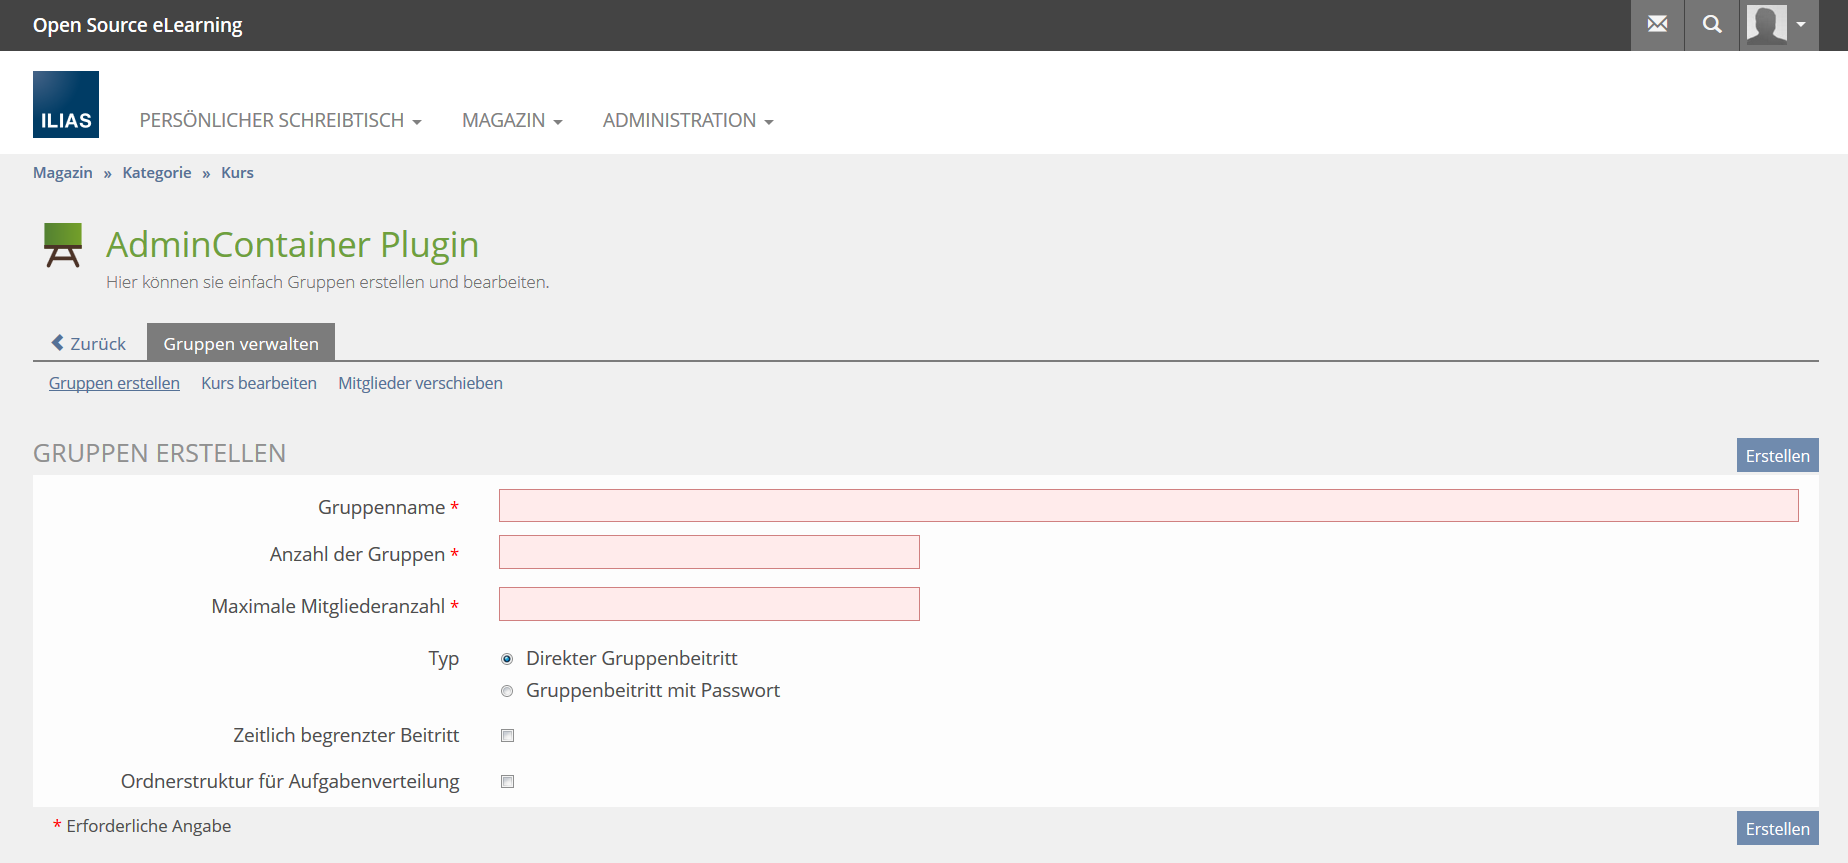
\includegraphics[width=1\textwidth]{img/gruppenErstellen.png}
	\caption{Ansicht Gruppen erstellen}
\end{figure}

allgemeiner Text zu Gruppen erstellen
\subsection*{Unterpunkt}
\begin{itemize}
	\item Text Unterpunkt
\end{itemize}

\clearpage

\section{Kurs bearbeiten}
\begin{figure}
	\centering
	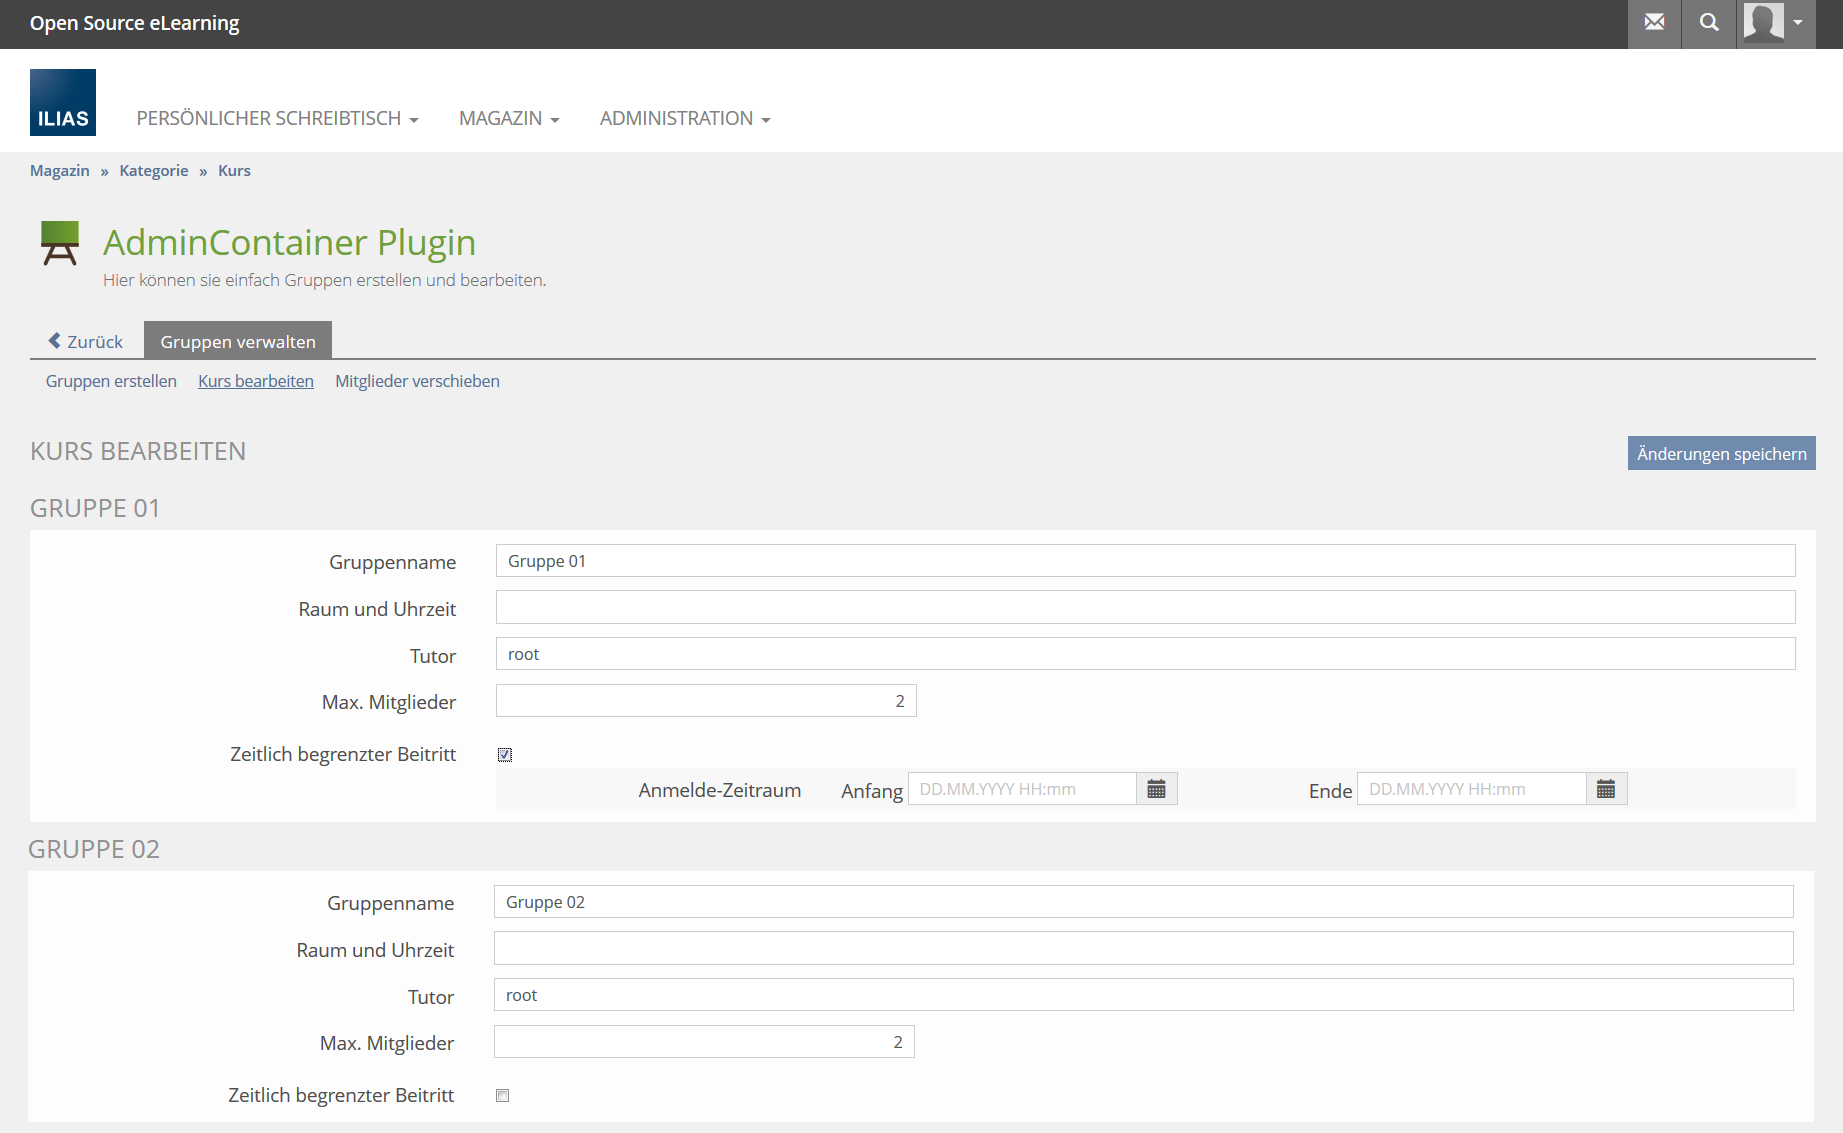
\includegraphics[width=1\textwidth]{img/kursBearbeiten.png}
	\caption{Ansicht Kurs bearbeiten}
\end{figure}

allgemeiner Text zu Kurs bearbeiten
\subsection*{Unterpunkt}
\begin{itemize}
	\item Text Unterpunkt
\end{itemize}

\clearpage

\section{Mitglieder verschieben}
\begin{figure}
	\centering
	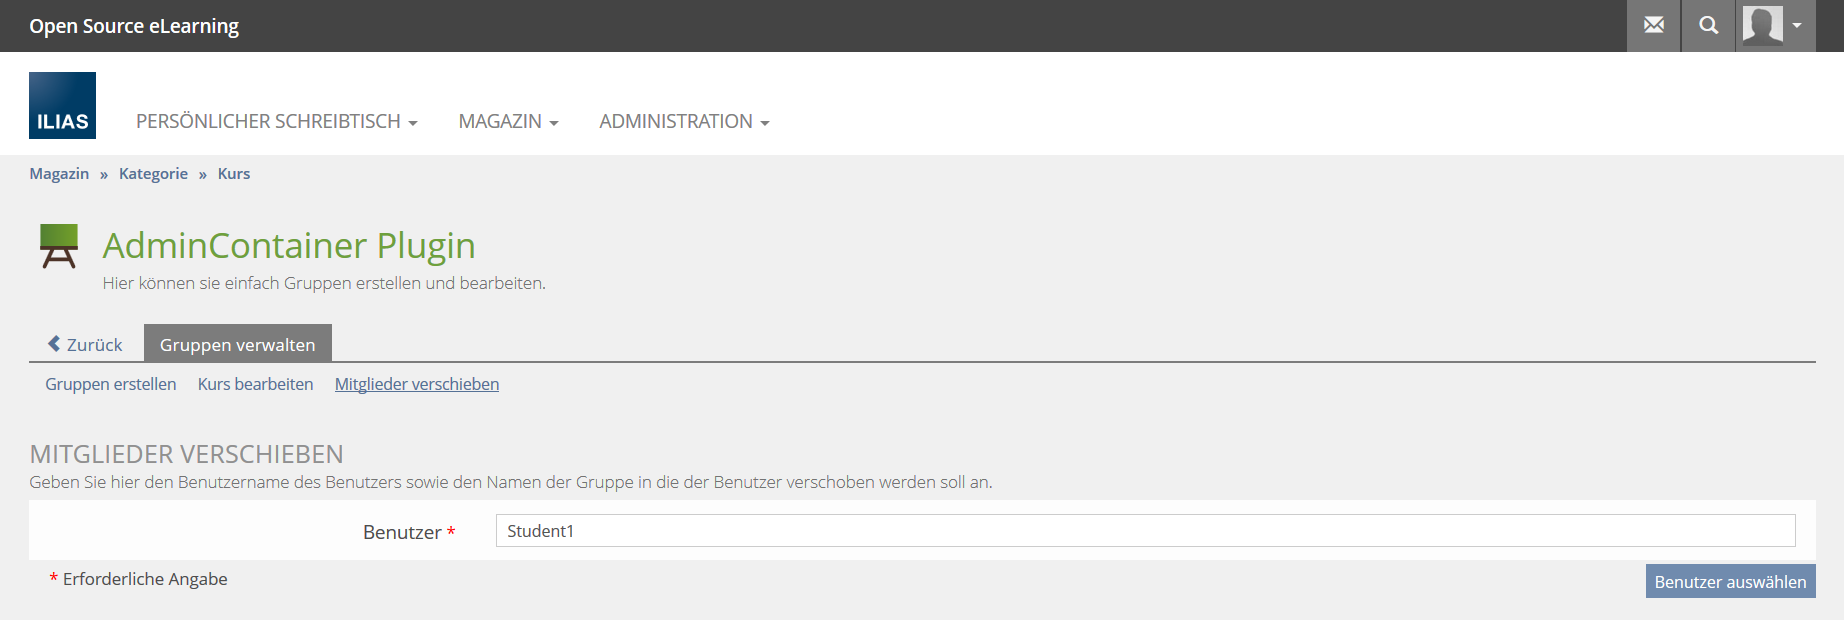
\includegraphics[width=1\textwidth]{img/mitgliederVerschieben.png}
	\caption{Ansicht Mitglieder verschieben}
\end{figure}

allgemeiner Text zu Mitglieder verschieben
\subsection*{Unterpunkt}
\begin{itemize}
	\item Text Unterpunkt
\end{itemize}

\clearpage